%%\documentclass[aps,prb,floatfix,showpacs,preprint]{revtex4}
\documentclass[aps,prl,floatfix,twocolumn]{revtex4-1}

\usepackage{epsfig}
\usepackage{verbatim}	 % for block comments \begin{comment} \end{comment}
\usepackage{amssymb}
% \usepackage{bbold}
\usepackage{bm}
\usepackage{amsmath}
\usepackage{psfrag}
\bibliographystyle{apsrev}
\usepackage{color}
% \usepackage{ulem}
\usepackage[latin1]{inputenc}
\usepackage[english]{babel}
\usepackage{graphicx}
\usepackage{amscd}
\usepackage{eucal}
\usepackage{bm}
%\usepackage{pslatex}
\usepackage{hyperref}
\usepackage{lipsum}
\usepackage{mathtools}
\usepackage{multirow}
% \usepackage{natbib}
\usepackage{todonotes}

\begin{document}

\title{The K-player: some authors beat the power law}

\author{A. B.\textsuperscript{1,2}, M. N.\textsuperscript{2,3}, and X. Y.\textsuperscript{3,1}}
% \author{R. Delabays\textsuperscript{1,2} and M. Tyloo\textsuperscript{1,3}}
\affiliation{\textsuperscript{1} Concordia Research Station, Antarctica. \\
\textsuperscript{2} International Space Station (ISS), Low Orbit. \\
\textsuperscript{3} Professor Khromov, Research Vessel, Arctic Ocean.}
% \affiliation{\textsuperscript{1} School of Engineering, University of Applied Sciences of Western Switzerland HES-SO CH-1951 Sion, Switzerland. \\
% \textsuperscript{2} Automatic Control Laboratory, Swiss Federal Institute of Technology (ETH) Z\"urich,  Switzerland. \\
% \textsuperscript{3} Institute of Physics, EPF Lausanne, CH-1015 Lausanne, Switzerland. }

\date{\today}

\begin{abstract}
 \textcolor{red}{\lipsum[1]}
\end{abstract}

\maketitle

\section{Introduction} 

\todo[inline]{Re-write intro}

As pointed out by Sekara et al.~\cite{Sek18}, publishing in a peer-reviewed journal is more likely if one author of the manuscript already published in the same journal.
An outcome that could be expected of such an observation is a high representation of a few authors in a given journal. 

In line with this, a scientist whose research topic is well-aligned with a journal topic is likely to publish a large proportion of their work in this journal.
Leading to a high representation of this author. 

In this manuscript, we support these expectations, showing that in a selection of \textcolor{red}{twelve} journals, the distribution of the number of authors with respect to the number of articles published within a journal is close to a power-law, and in particular has a heavy tail. 
Furthermore, we observe that whereas in general this distribution has a slightly thinner tail than a power-law, in some journals, there exists a few authors whose number of publications is significantly larger than what the power-law would predict. 
We refer to those authors as \emph{K-players} to emphasize their preponderant role in the journal. 

We relate this power-law-like distribution to a mechanism that can be compared to \emph{preferential attachement} in the context of network evolution. 
It has been shown that such a mechanism of network construction leads to a degree distribution that follows a power-law~\cite{Kra00}.

\begin{figure*}
 \centering
 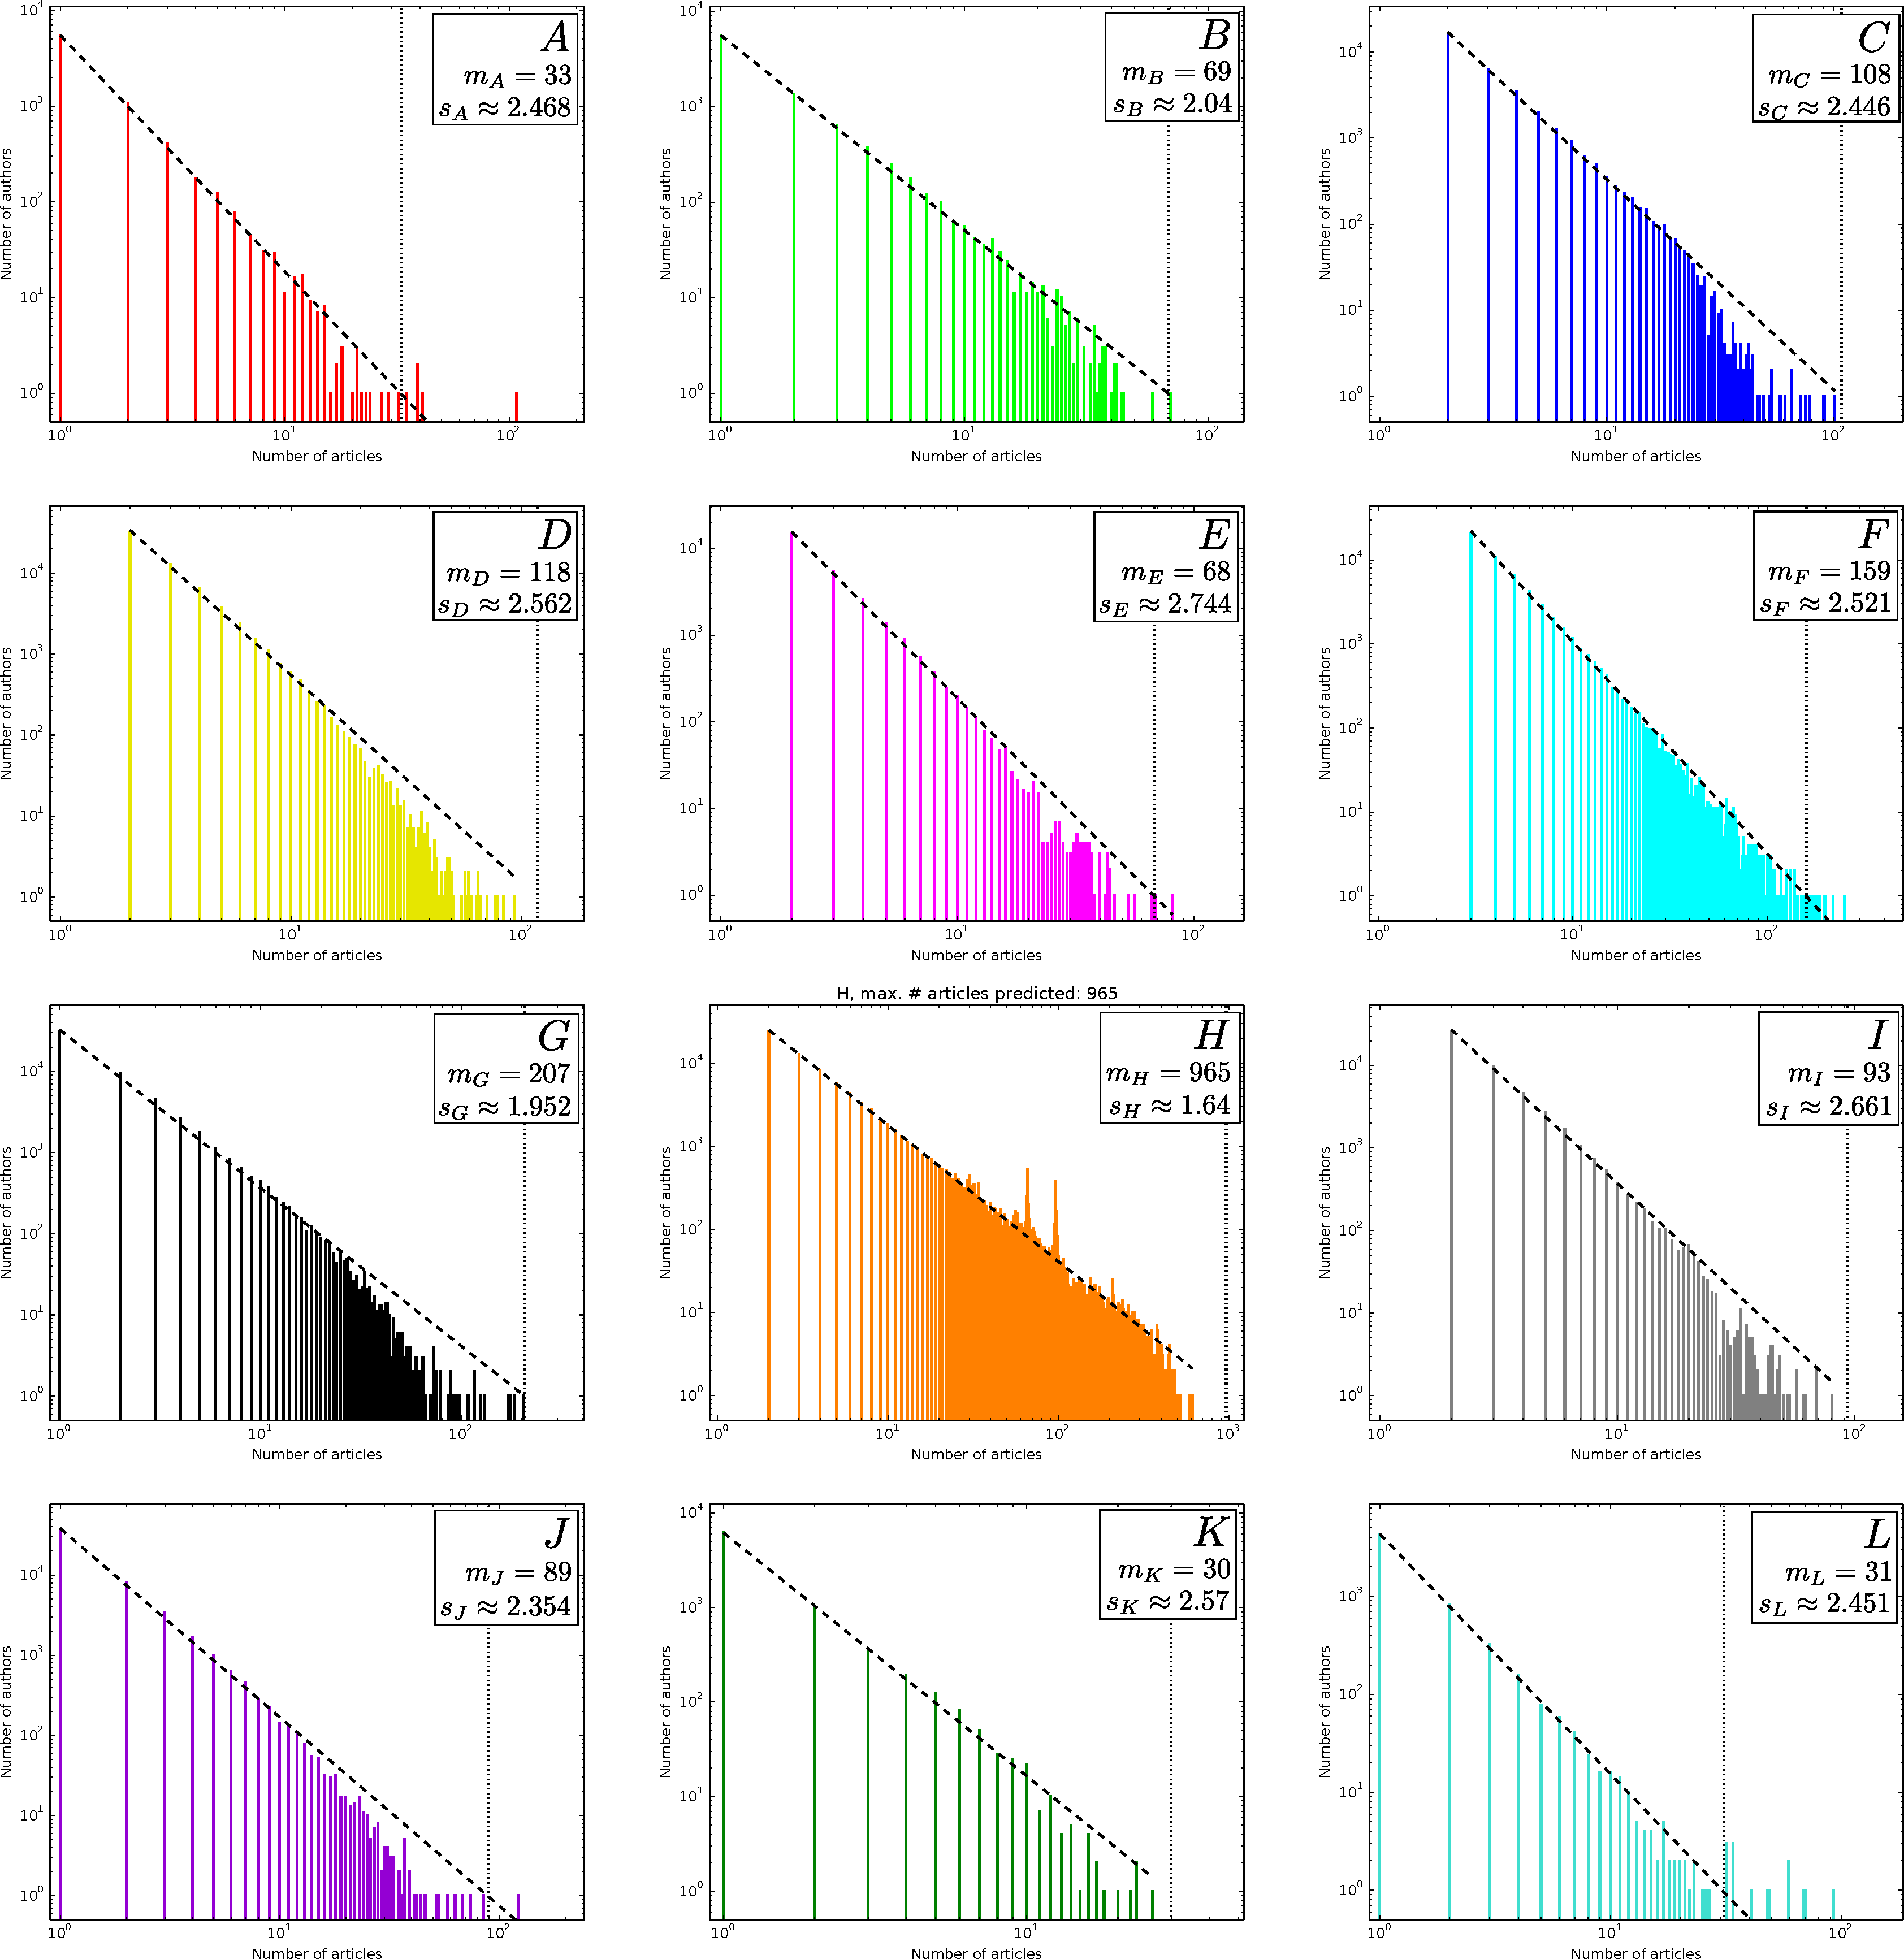
\includegraphics[width=\textwidth]{figures/ABCDEFGHIJKL.pdf}
 \caption{Blah...}
 \label{fig:1}
\end{figure*}

\section{Methodology}
We consider an arbitrary selection of 12 peer-reviewed journals (see Table~\ref{tab:journals}), whose data are available on the Web of Science database (WoS)~\cite{WoS}. 
Each journal considered is sufficiently old (at least \textcolor{red}{20 years???}) and is still publishing articles nowadays. 
We denote by ${\cal J}\coloneqq\{{\rm BMJ},{\rm CHA},...,{\rm TAC}\}$ the set of journals considered.

\begin{table}
 \begin{tabular}{l|l|l}
  & Label & Journal name \\
  \hline
  \hline 1 & BMJ & British Medical Journal \\
  \hline 2 & CHA & Chaos \\
  \hline 3 & ENE & Energy \\
  \hline 4 & LAN & The Lancet$^*$ \\
  \hline 5 & NAT & Nature$^*$ \\
  \hline 6 & NEG & New England Journal of Medicin$^*$ \\
  \hline 7 & PNA & Proceedings of the Natural Academy of Sciences$^{**}$ \\
  \hline 8 & PRD & Physical Review D \\
  \hline 9 & PRL & Physical Review Letters$^*$ \\
  \hline 10 & SCI & Science$^*$ \\
  \hline 11 & SCM & Scientometrics \\
  \hline 12 & TAC & IEEE Transactions on Automatic Control 
 \end{tabular}
 \caption{Labels and names of the journals considered. 
 Journals where the authors with one (resp. two) articles published were discarded are indicated by $^*$ (resp. $^{**}$).}
 \label{tab:journals}
\end{table}

Within each journal ${\rm JOU}\in {\cal J}$ and for each author $i$ who published in ${\rm JOU}$, we count the number $n^{\rm JOU}_i$ of articles published by $i$, which gives the set of data $N_{\rm JOU}=\{n^{\rm JOU}_i\}$. 
We restricted our investigation to publications labelled as ``Article'' in the WoS database, to focus on peer-reviewed articles and to discard editorial material. 
For some journals, the number of authors was too large to be downloaded from the Web of Science database. 
As a consequence, some authors having published only one or two articles in these journals had to be removed from the data (e.g., ${\rm PRL}$). 
When this happens, it is indicated by asteriscs in Table~\ref{tab:journals}.
Note also that we did not take into account articles published anonymously, which represent a large number of articles in medicine journals in particular. 
\textcolor{red}{Do the same for the time-splitted data !!!}
From these data, within each journal ${\rm JOU}\in{\cal J}$, we can compute for each number of articles published $n$, the number of authors who published $n$ articles 
\begin{align}
 a_{\rm JOU}(n)\coloneqq\#\{i\colon n^{\rm JOU}_i = n\}\, ,
\end{align}
The distributions of this value are represented in logarithmic scales in Fig.~\ref{fig:1}, each panel corresonding to a different journal. 

To the eye, these distributions have a heavy tail and it is tempting to fit a power law to it, 
\begin{align}\label{eq:pl}
 \mathbb{P}_{\rm pl}(a = n) &= C_1\cdot n^{-\alpha}\, .
\end{align}
However, as pointed out by Broido and Clauset~\cite{Bro18}, caution is needed when fitting a power law to heavy tailed data. 
Thus we also tried to fit other heavy tailed distributions, the \emph{power law with cutoff}~\cite{Bro18} being one of them, 
\begin{align}\label{eq:plco}
 \mathbb{P}_{\rm plc}(a = n) &= C_2\cdot n^{-\beta}e^{-\gamma n}\, .
\end{align} 
We performed the distribution fitting by optimizing the parameters $\alpha$, $\beta$, and $\gamma$ with a Maximum Likelihood Estimator (MLE)~\cite{Cla09}. 

To evaluate the goodness of our fitting, we proceeded as follows. 
We generated $2500$ sets of synthetic data $D_i$, $i=1,...,2500$, following the distribution obtained. 
Comparing our data $D_0=\{a_{\rm JOU}(n)\}$ to the sets of synthetic data, we can compute $p$, the proportion of synthetic data that are further than $D_0$ 
(in the Kolmogorov-Smirnov sense~\textcolor{red}{REF}) from the theoretical distribution. 
The fit is considered as \emph{good} if $p>0.05$. 


\section{Results}
The results of each fit and goodness-of-fit tests are presented in Table~\ref{tab:fit_gof}. 
Clearly, the power law distribution is a poor fit for all data, its $p$-value being (almost) zero for all journals. 
This can be seen in Fig.~\ref{fig:1} as for most of the journals, the tail of the data set is lighter that the tail of its power law fit (black dashed line). 
However, for some journals \textcolor{red}{(namely BLI, BLA, BLO)}, the $p$-value of the power law with cutoff is high and it seems to be a rather good fit (black dotted line in Fig.~\ref{fig:1}). 

\begin{table}
 \begin{tabular}{l|l||c|c||c|c|c}
  && \multicolumn{2}{c||}{PL} & \multicolumn{3}{c}{PL with cutoff} \\
  && $\alpha$ & $p$ & $\beta$ & $\gamma$ & $p$ \\
  \hline
  \hline 1 & BMJ & &&&& \\
  \hline 2 & CHA & &&&& \\
  \hline 3 & ENE & &&&& \\
  \hline 4 & LAN & &&&& \\
  \hline 5 & NAT & &&&& \\
  \hline 6 & NEG & &&&& \\
  \hline 7 & PNA & &&&& \\
  \hline 8 & PRD & &&&& \\
  \hline 9 & PRL & &&&& \\
  \hline 10 & SCI & &&&& \\
  \hline 11 & SCM & &&&& \\
  \hline 12 & TAC & &&&&
 \end{tabular}
 \caption{Fitted parameters and $p$-value of the goodness-of-fit for power law and power law with cutoff distributions.}
 \label{tab:fit_gof}
\end{table}

We tried to fit other heavy tailed distributions \textcolor{red}{(such as BLI, BLA, BLO)}, but none of them performed better than the power law with cutoff under our goodness-of-fit test. 


\paragraph{}
{\bf General explanation. }
The better explanation we found to this heavy tail behavior is the following. 
It has been \textcolor{red}{shown/postulated [REF]}, that the number of coauthorship of an author is ruled by \emph{preferential attachement}. 
Namely, the probability that an author will create a new scientific collaboration at time $t$ is proportional to the number of scientific collaboration they have. 
It is reasonable to assume that the evolution of the number of articles published by an author in a given journal is described by a similar preferential attachment process. 
In other words, it means the probability that a new article published in a given journal 
is signed by an author is proportional to the number of articles published by this author in the given journal. 

Heuristically, our argument is that if an author published a lot of article in a journal, it means (i) that they write a lot of papers, 
and (ii) that their research topic is well-aligned with the topics covered by the journal. 
Assumptions (i) and (ii) together imply that this author is likely to published again in this journal. 

To make this more rigorous, for three journals (BLI, BLA, and BLO) we compared the number of authors having published $k$ articles at year $t$ 
with the number of articles published by these authors between years $t$ and $t+1$. 
Defining $m_k(t,s)$ as the number of articles published between years $t$ and $s$ by the authors with $k$ articles at time $t$, we plot in Fig.~\ref{fig:2} the values of $m_k(t,t+1)/N_k(t)$ with respect to $k$ for years $t\in\{1999,...,2008\}$. 
For each of the three journals, these values have a linear correlation coefficient larger than $0.5$, supporting a fairly good linear dependence, 
\begin{align}\label{eq:prop}
 m_k(t,t+1) &\approx k\cdot N_k(t)\, . 
\end{align}
\textcolor{red}{Restrict the data to a time span of max. 30 years to remove authors who are not publishing anymore.}

\begin{figure*}
 \centering
 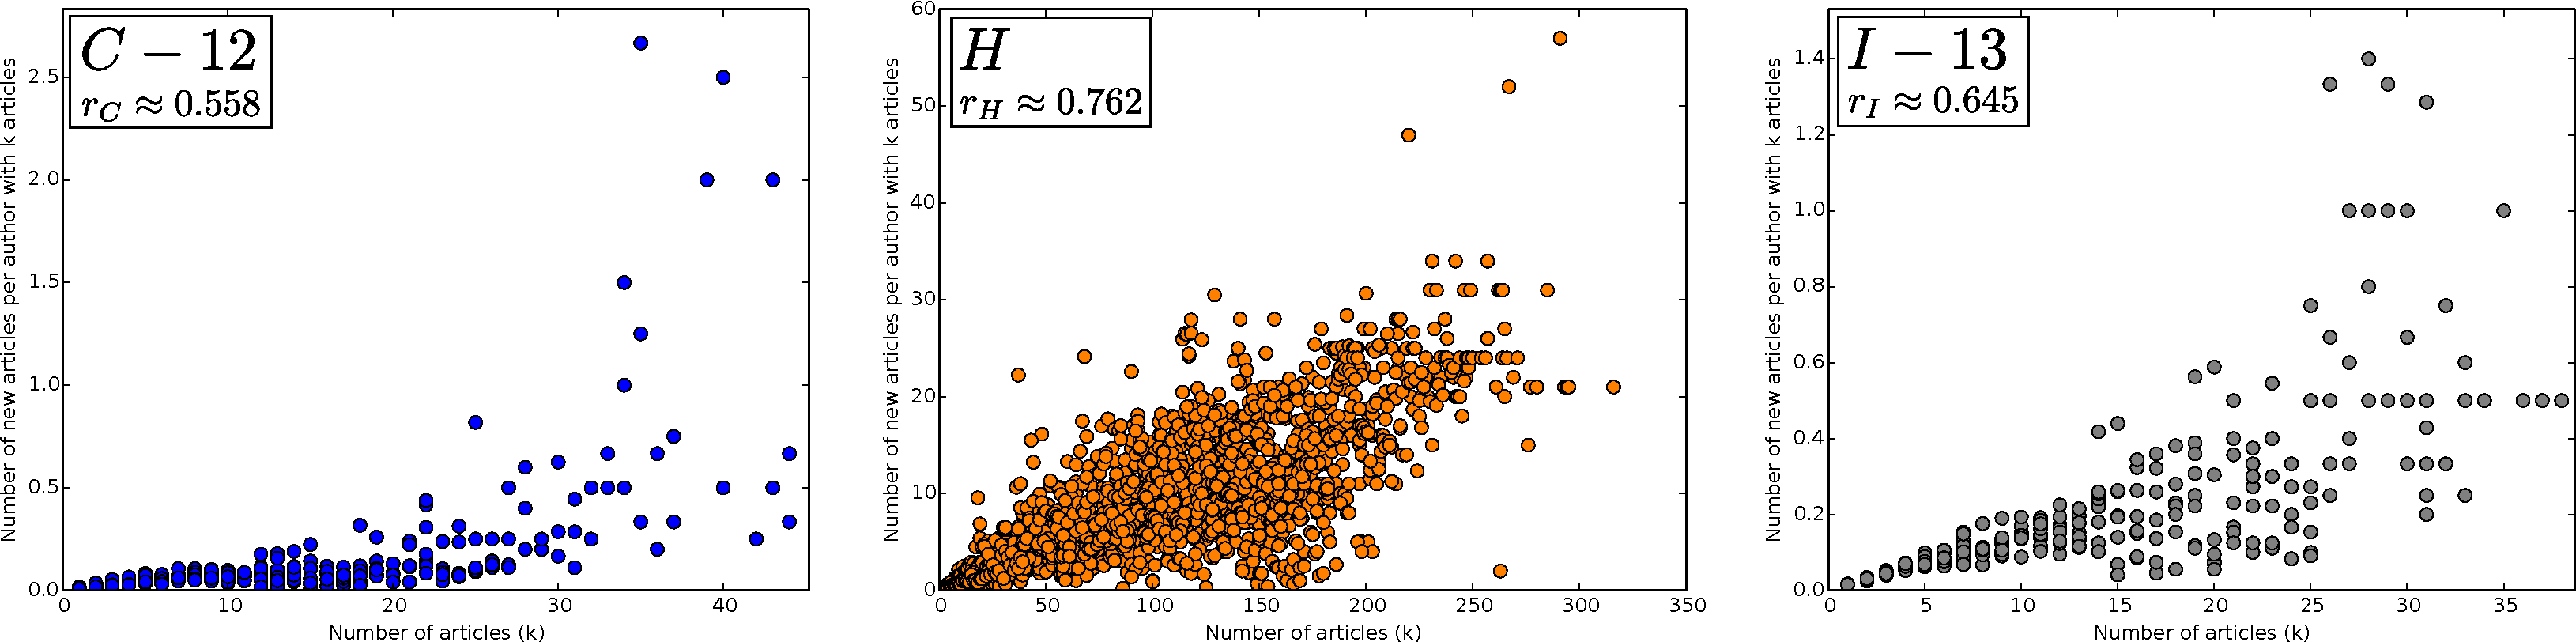
\includegraphics[width=\textwidth]{figures/CHI_correl.pdf}
 \caption{Blih...}
 \label{fig:2}
\end{figure*}

The probability that a new paper is signed by an author with $k$ publications is then close to be proportional to $k$. 
According to~\cite{Kra00}, if it was exactly proportional, after a long enough time, the distribution of $N_k$ would follow a power law. 
The fact that the relation~\eqref{eq:prop} is not exact and that our samples are limited to a finite time horizon, explain that we do not obtain exactly a power law. 
However, the good correlation between $m_k(t,t+1)/N_k(t)$ and $k$ tells us that the distribution should not be too far away from a power law, in agreement with our observation of a power law with cutoff.


\section{Observations}
Aside of these general considerations, we note two interesting observations in the data. 
Namely, some authors are stronger that the power law, and some very large experiments can be seen even in aggregated data. 

\subsection{Exceptions }
The general distribution of the number of authors with respect to the number of paper per author is quite clear in our analysis. 
However, in some journals, we observe anomalies (see journals \textcolor{red}{BLI,BLA, and BLO} in Fig.~\ref{fig:1}). 
It appears that sometimes, some authors publish significantly more articles in a journal than what the power law with cutoff would predict, and somtimes even more articles that what a power law would predict. 
These authors, who we refer to as \emph{K-players}, are supposedly some very influencial scientists in the journal considered, and they literally \emph{beat the power law}.

\paragraph{}
{\bf Remark.}\textit{
We emphasize that we checked that these K-players are not artifacts due to multiple authors having the same name which would count as the same person. 
In all cases presented here, there is a unique person appearing in the authors' list of a very large number of papers. 
}

\subsection{Peaks in PRL and PRD}
We observe two peaks in the distribution of PRL (around 70 and 96) and PRD (around 77 and 104). 
Crossing the lists of authors for each number of articles between 63 and 102 (resp. 72 and 111) for PRL (resp. PRD), we get Fig.~\ref{fig:prl_prd}. 
The fact that the authors composing a peak in PRL are the same composing one of the peaks in PRD suggests that these authors are all part of a large group publishing together. 
After a quick search, we realize that the peaks correspond to the research groups of the experiments ATLAS and CMS at the  \emph{Centre Europ\'een de Recherche Nucl\'eaire} (CERN). 
\begin{figure}
 \centering
 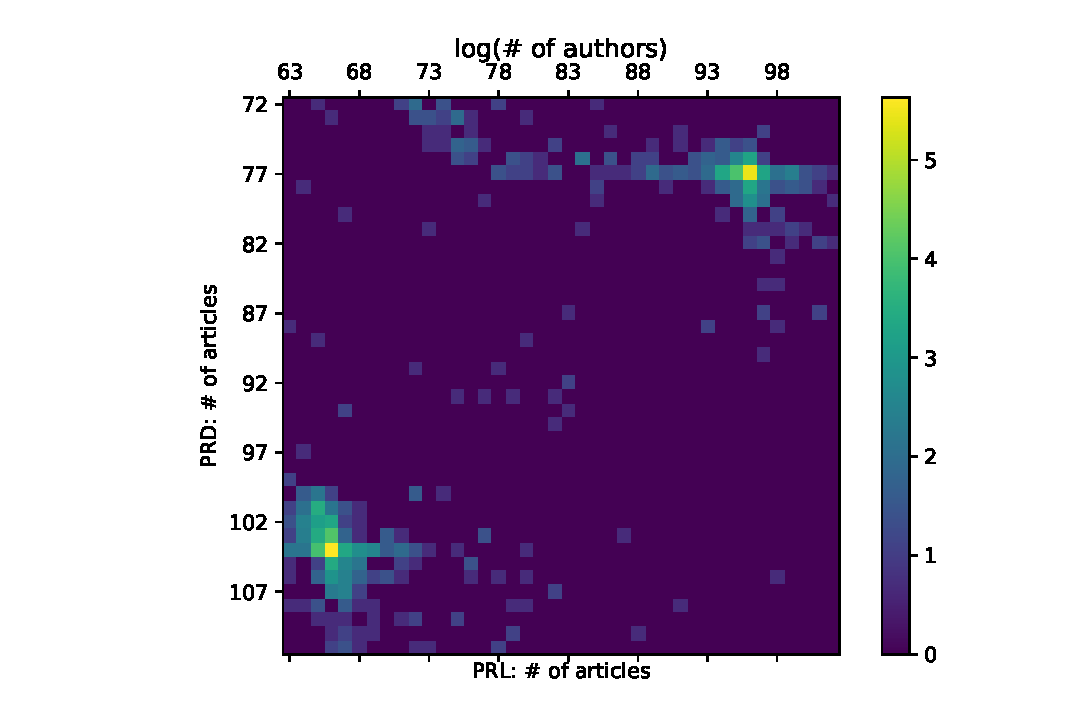
\includegraphics[width=.8\columnwidth]{figures/prl_prd_log.pdf}
 \caption{Beuh.}
 \label{fig:prl_prd}
\end{figure}
These two experiments are so big that they can be seen, even in the aggregated data used in our analysis. 

\section{Conclusion}


\bibliographystyle{apsrev4-1}
\bibliography{bibliography}

\end{document}
